\chapter{Methodology}
\label{chap:methodology}

In order to address the research questions, we wanted to develop a proof of concept system that is able to investigate and utilize the concepts in question. It was decided that a to-do list application would be a good candidate for investigating these concepts. A to-do list application is a task management system in a simple form. The simplest version of it could be just a list of strings representing the user's tasks, or to-do items, that needs to be done. Another form of a task management system is a calendar. A calendar would also be a suitable candidate for looking into the use of contexts in task management. However, a calendar is more complex than a to-do list, even in its simplest form, and would require more design decisions than a to-do list if building a system from scratch. Considering this, a to-do list application was chosen.

By designing a to-do list application, we want to discover the important decisions that needs to be made when developing such an application, both in terms of architecture as well as graphical design. We also want to discover how to make such an application context-aware, and how contexts can be used towards a meaningful purpose in such a system. This involves how to collect the contexts, how to store them, and also how to represent them so that they can be used.

When building context-aware systems, the most natural choice of platform is mobile devices. Contextual information is readily available on such devices because of their cheap and integrated sensors, which now exists on nearly all modern handheld devices. It is easy to access information such as user activity, time and location. The two most popular operating systems for such devices are Android and iOS. The development frameworks for both of these have functionality that allows developers to easily collect contextual data in their applications. Even context abstraction and representation are handled by the frameworks, so that the developer no longer has to deal with the raw sensory data coming from the hardware. For this particular thesis, the Android Operating System was chosen for development. This is mostly because it holds the biggest market share by far, but also because an Android device was easily available for development.




\section{User group}
In our application we decided that using a recommender to recommend tasks from the users to-do list based on contexts was one way of utilizing contexts in such an application. For the recommender to be able to differ between user tasks, these tasks needs to be assigned different types and be categorized. However, categorizing typical and everyday tasks will require a lot of effort. It is known that modeling an individual's tasks and activities can be challenging \cite{refanidis2010constraint}. Consider trying to generalize the tasks of an office worker and a carpenter. The tasks that these two typically do during a day, will vary greatly. Finding similarities among these tasks so that they could be generalized to fit a general population would be difficult. Therefore, in order to reduce complexity and the amount of work needed, it was decided that the scope should be narrowed down by selecting a specific user group. This will also allow for narrowing down the application itself, both in terms of general application design as well as the complexity of context collection and representation.

The user group that was selected was students, and more specifically students in an educational environment. There were two main reasons for this. One being that the tasks of such a narrowed down and specific user group can be much easier divided into separate types and categorized. We will then be able to predefine a set of tasks that should cover most of the different types of tasks that a student will be doing in an educational environment. The second reason for choosing students was that this user group was easily accessible, both for handing out questionnaires and also for seeking participants for an experiment.

Although students were selected as the target user group, typical educational tasks can still vary to a large degree between undergraduate and postgraduate students. This can also be highly dependent on what semester the student in question is currently in. A bachelor student might have very different tasks than a master student doing his/her master thesis. To determine these differences, and to find out whether or not such differences needed to be accounted for in the application design, a short questionnaire was made. Detailed results of the questionnaire can be found in Section~\ref{subsec:studenttasks}. Through the questionnaire, we found that there were only minor differences between the tasks of the different types of students. It was therefore decided that the tasks should be categorized equally for all students.

The actual task categories used for the tasks in the application were:
\begin{itemize}
	\item Attend lecture
	\item Read
	\item Write report
	\item Do course exercises
	\item Meeting
	\item Group work
	\item Practical work
	\item Other
\end{itemize}
These categories are based on the results of the short student task questionnaire we made. We provided a set of predefined tasks where the student had to answer how often they typically performed each task, both in terms of regularity (once a day, once a week etc.) and frequency (1-3 times a week, 4-6 times a week etc.). The reason we distinguished between frequency and regularity is that we wanted to catch if a user did a typical task irregularly (once a month), but then quite often during that period (multiple times per day, once a month, for example). The students were also able to fill in additional tasks, if the predefined tasks were not enough to cover all the tasks that they typically do.



\section{Application}
\label{sec:application}

\subsection{General application design}
By choosing to create a todo-list application, the user should be able to perform actions that are normal for such applications. These actions include creating and storing tasks, as well editing and deleting them. It should also be possible to organize the tasks by arranging them into lists. By studying other to-do list applications \cite{trello, todoist} we came up with a set of minimum requirements that the application would have to fulfill.
\begin{itemize}
	\item Creating tasks.
	\item Editing/deleting tasks.
	\item Creating lists for tasks.
	\item Managing lists by editing/deleting them, or moving tasks between lists.
\end{itemize}
These are core features that are supported in popular to-do lists, and the users would expect a to-do list to have this functionality. The application in this study is developed in a way that supports all these aspects. When a todo-item or task is created, a date will be attached to that particular task, thereby organizing the tasks with similar dates into lists.

We want to utilize context features in our application in order to make task recommendations for the user. Therefore, we would have a few more requirements in addition to the ones mentioned above:
\begin{itemize}
	\item Collection of contexts
	\item Modeling and representing the contexts in a way that they can be utilized.
	\item A recommender module to process the tasks and contextual information.
\end{itemize}

With the above requirements in mind, we designed a conceptual model of the application, shown in Figure~\ref{fig:conceptualmodel}.
\begin{figure}[tbp]
  \centering
  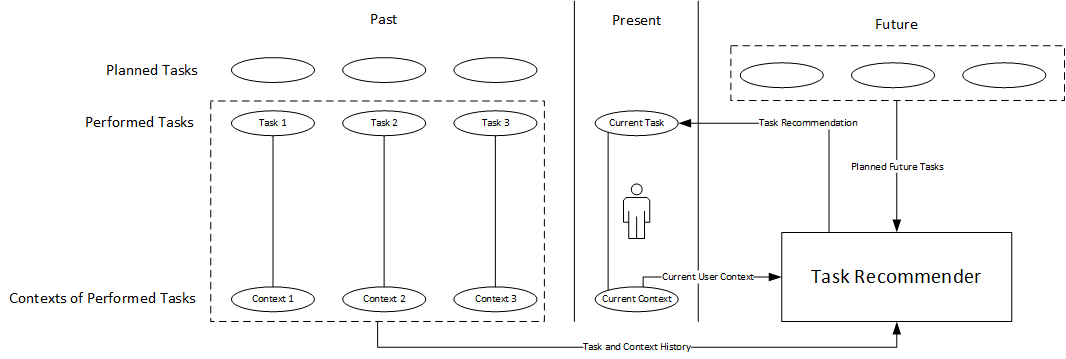
\includegraphics[width=\textwidth]{figures/ConceptualDiagram.png}
  \caption[Conceptual model]{Conceptual model of the application.}
  \label{fig:conceptualmodel}
\end{figure}
The figure shows the general idea behind the application. We have the user in the center with a current context. On the top right we have all the tasks that the user has planned to do in the application. When a user selects one of these tasks and starts doing the task, the mobile device will continuously collect information about the users contexts. Contexts are collected for as long as the user is actively performing the task. When the user tells the application that he/she is finished with a task, all the collected contexts are stored together with the task in the database, as shown on the left side of the figure (dotted lines). Here, the completed tasks and their related contexts make up the task and context history.

The recommender is a separate and independent module in the application. The lines pointing towards the recommender represents its input, whereas the line pointing outward is the output, i.e. the actual task recommendation. The input for the recommender consists of three parts:
\begin{itemize}
	\item The tasks that the user needs to do (planned tasks).
	\item The tasks that the user has previously done (task history) and the contexts related to these tasks (context history).
	\item The users current context.
\end{itemize}
By taking all these components into account, the recommender will be able process the information and suggest a task and a task ordering for the user. The recommender part of the application is discussed more thoroughly in Section~\ref{sec:recommender}.

In the overall design of the application, we decided to stay with the Android design principles\cite{androiddesign} as much as possible. Popular apps on Google Play tend to follow similar design patterns, which means that Android OS users are accustomed to a certain look and feel. We wanted to provide a look and feel in our application that would be familiar to the users, in this case the students using the application. The graphical design of the main application screen is shown in Figure~\ref{fig:designmainscreen}.
\begin{figure}[tbp]
  \centering
  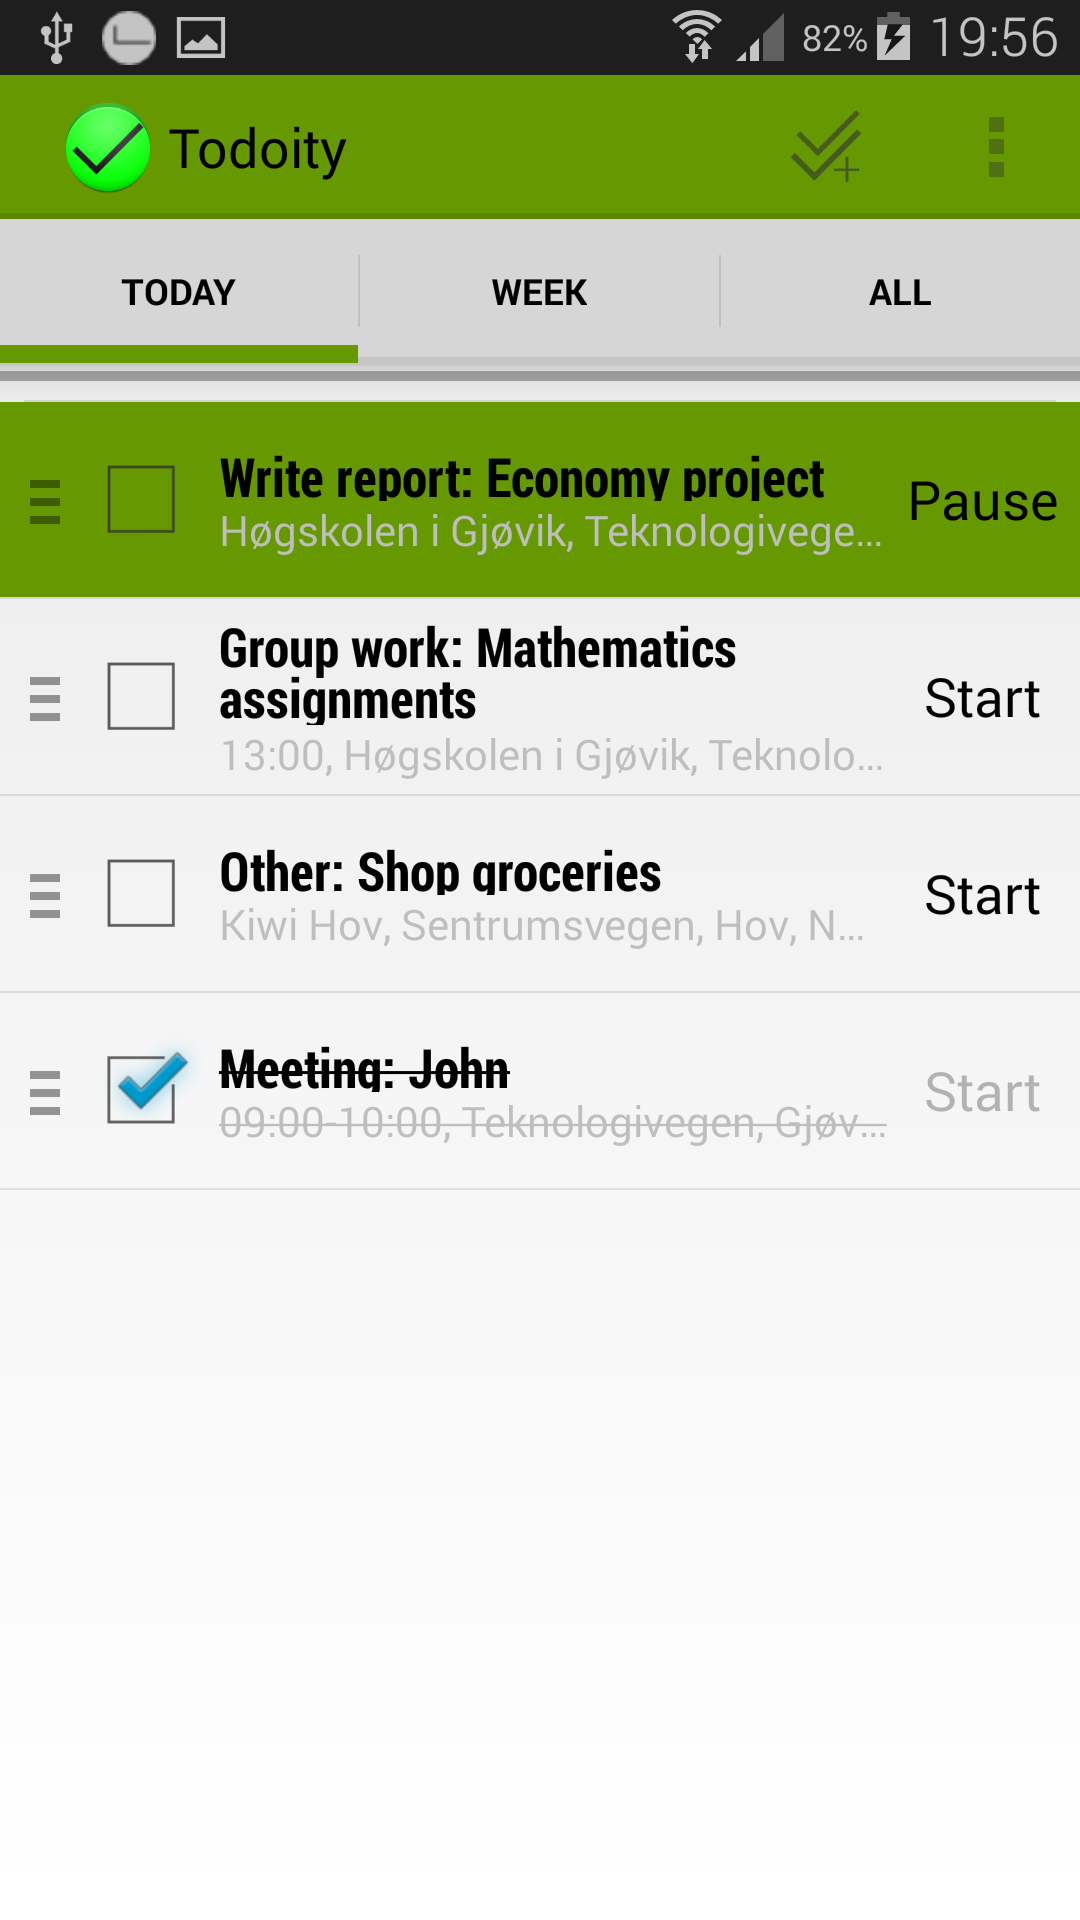
\includegraphics[width=0.35\textwidth]{figures/MainScreenStarted.png}
  \caption[Main application screen]{The main screen of the application, showing a few tasks where one is ongoing and one is finished.}
  \label{fig:designmainscreen}
\end{figure}
Here we can see several similarities with the design guidelines. There is a toolbar with common actions at the top (new task button and an overflow menu with settings and about) which is also given a app-specific color that runs through several other parts of the application (also called branding). We also provided tabs to allow the users to easily change between viewing both future planned tasks and past tasks. The \emph{today} tab is the default tab, displaying the tasks that the user has planned for the current day. Tasks that have been started by the user is placed at the top of the list and given a background color to indicate that it is running. Finished tasks are automatically placed at the bottom. The user also have the option to reorder the tasks through drag and drop.

A slightly simplified version of the overall workflow of the application is shown in Figure~\ref{fig:workflow}.
\begin{figure}[tbp]
  \centering
  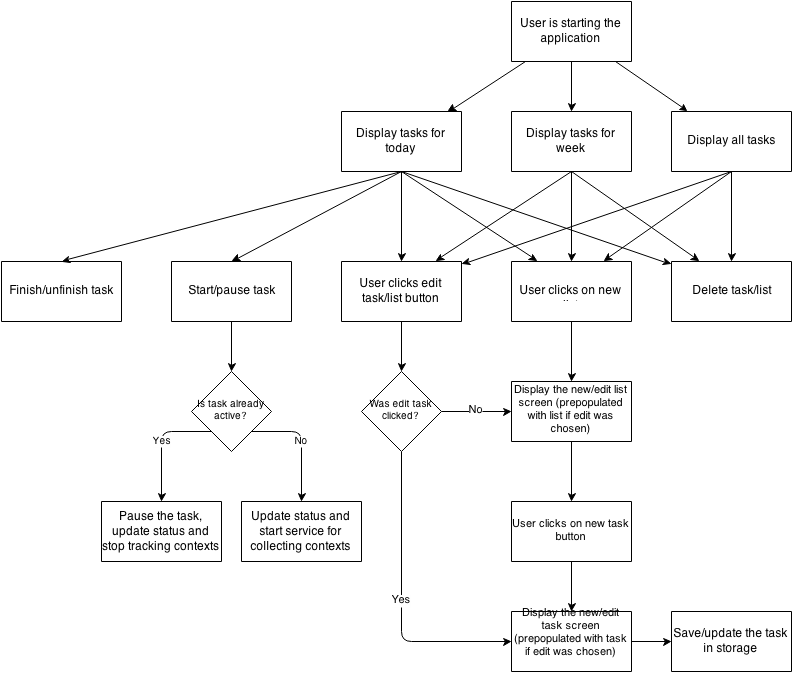
\includegraphics[width=0.7\textwidth]{figures/Workflow.png}
  \caption[Application workflow]{Application workflow.}
  \label{fig:workflow}
\end{figure}
This depicts the basic functionality that is provided. 

When the users launches the application, the \emph{today} screen is shown by default. From here, the user can create a new list of tasks, add tasks to current lists or delete tasks or lists. Upon selecting a list, the user can edit and delete existing tasks within that list or create new tasks. When wanting to edit or create a new task the user is directed to the new task screen. This is where the actual information about the task is entered. The creation of a new task is shown in Figure~\ref{fig:newtask}.
\begin{figure}[tbp]
  \centering
  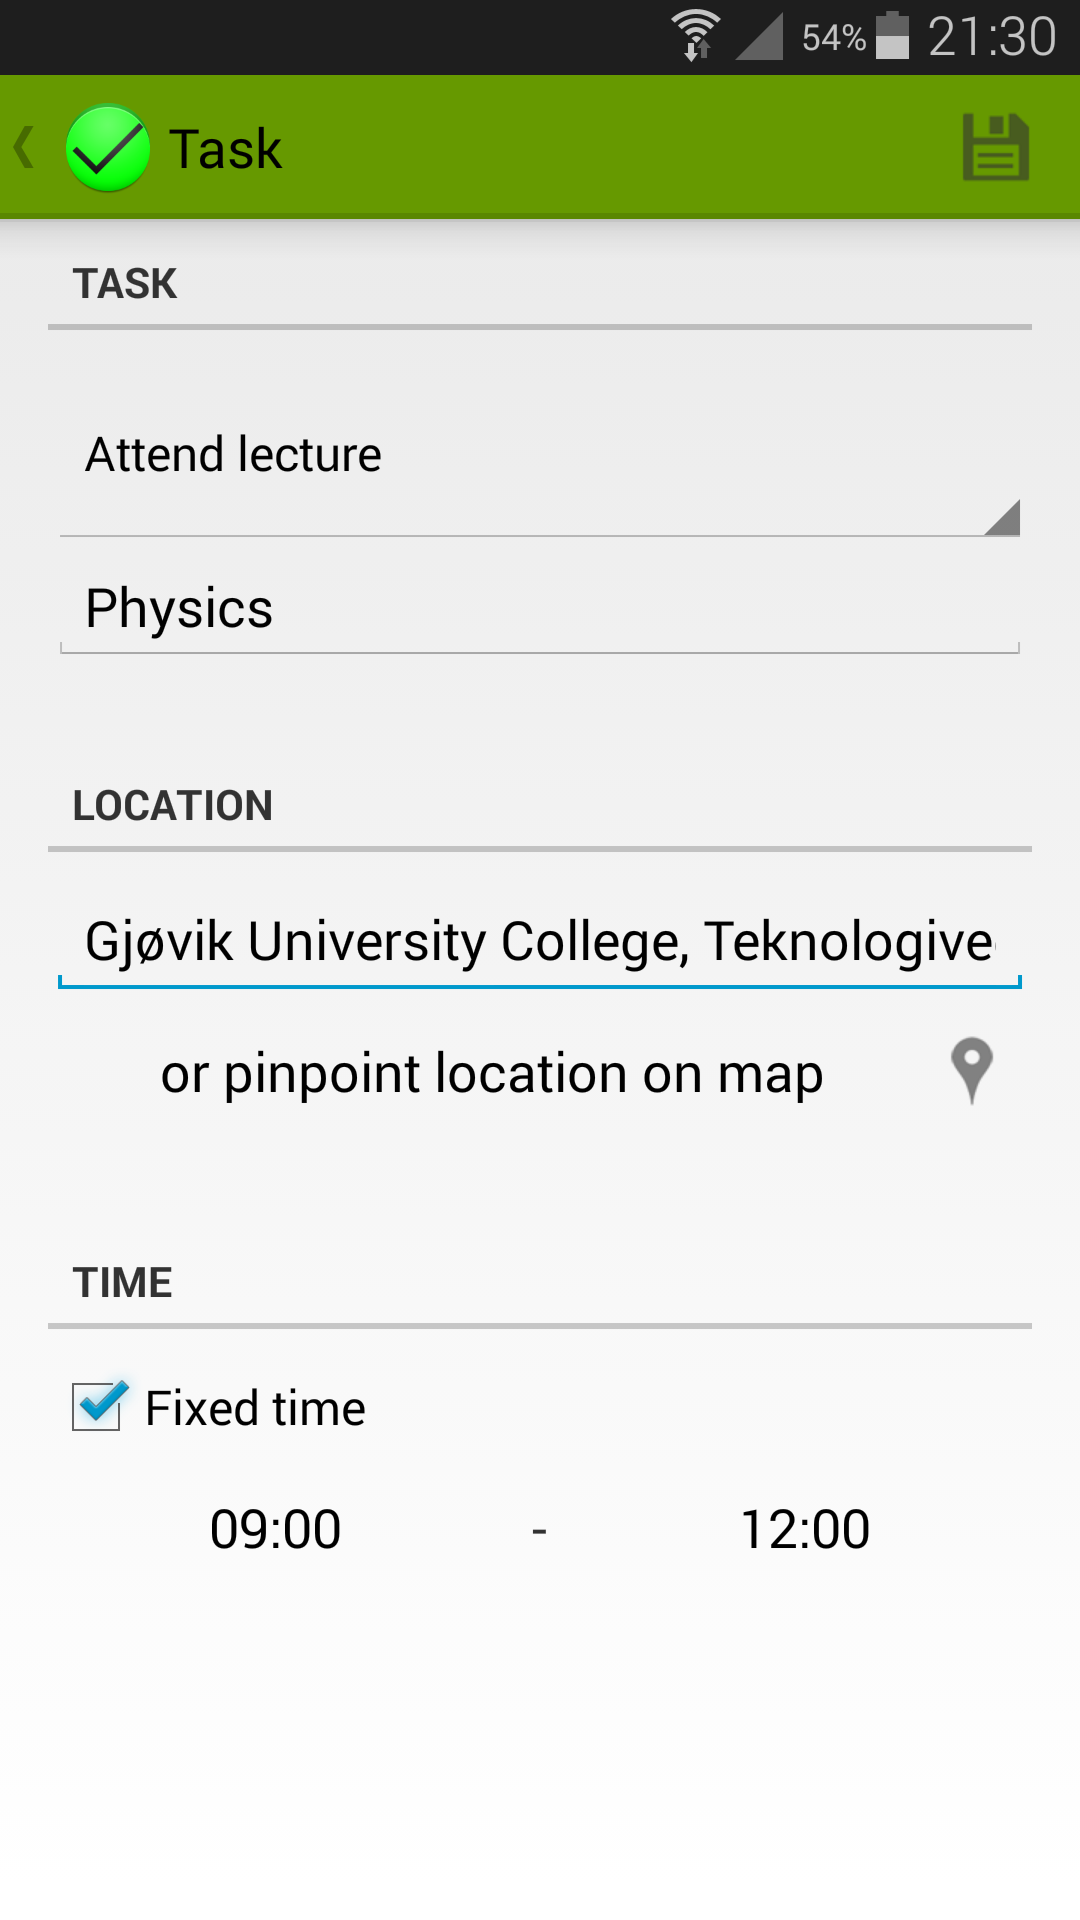
\includegraphics[width=0.35\textwidth]{figures/NewTask.png}
  \caption[Screen for creating a new task]{Creating a new task.}
  \label{fig:newtask}
\end{figure}
A category for the task has to be entered here. This is done by selecting one of our predefined tasks from a list. The user can also provide an optional description for the task. For this thesis, it was decided that a location should also be required by the users to provide. This is because we are designing a context-aware application that heavily relies on location. However, for a commercialized version of the application, a location would probably not be required as the users might get tired of having to input a location for every task. The location can either be input as text, where an autocomplete function was implemented to help users select real locations, or the map button can be clicked, which lets the user pinpoint the location from a map. The tasks can also have a fixed starting time and/or end time, which is optional.

\subsection{Collecting context information}
By storing contextual information about how tasks are performed, the recommender will be able to not only provide recommendations based on current and planned contexts, but also take into account in what contexts tasks have been done previously. A certain task may work well in one context and poorly in another. For example, if a user always perform one specific task in one specific context, such as always doing \emph{attend lecture} at campus, it would be meaningless to recommend this task if the user is at home. Before designing the overall schema of context representation, decisions on what contexts to actually use and collect in the application needs to be made. 

Although a whole variety of different contexts may be collected by a mobile device, not all of them would be equally relevant to use in a to-do list application. While most contexts could be used to some degree, there are situations were some contexts would be redundant. Humidity, for example, could be a somewhat useful context for someone working on very specific tasks in very specific environments, say an environmentalist taking water samples near lakes and rivers. However, for students in an educational environment, such contexts are less relevant. Because of this, the actual contexts that was decided to be collected in this application were:
\begin{itemize}
	\item \emph{Location:} Both the planned location of the task as well as the actual location of where the task is performed is stored.
	\item \emph{Activity:} The movement of the device while contexts are collected.
	\item \emph{Time:} Each task is given timestamps both when they are started and ended. By doing this it is possible for the recommender to separate tasks that are done at specific times of the day, week or even month. Time spent doing a task is also tracked, as this may differ from the difference between the start and end times (users may pause doing a task).
\end{itemize}
These are the ones we considered to be the most relevant for students in an educational environment. While other contexts, such as ambient sound, may be quite relevant for some tasks, such as reading, we decided not to implement the use of these contexts in our application. It would be interesting from a researching point of view to look at as many different contexts as possible, but given the timeframe of this thesis and the amount of work needed to implement them, we reduced the number of used contexts to the ones mentioned above.

The actual logic behind the tracking of tasks and their contexts is a separate problem. It was decided that the tracking of tasks would have to be manually started and stopped by the users. This was done by providing a start button for each task, as shown in Figure~\ref{fig:taskrepresentation}.
\begin{figure}[tbp]
  \centering
  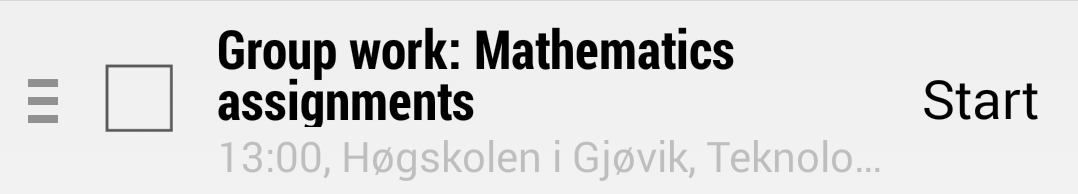
\includegraphics[width=0.5\textwidth]{figures/TaskRepresentation.png}
  \caption[In-app representation of task]{The in-app representation of a planned task.}
  \label{fig:taskrepresentation}
\end{figure}
The process of collecting contexts when the user is performing a task would ideally be done autonomously by the application, without letting the user be responsible for starting and stopping the tasks. However, there are difficulties in making this happen, which is discussed in Section~\ref{sec:contextcollectiondiscussion}. When the user starts a task, the application indicates to the user that something is happening in the background. This is done by highlighting the tasks for which contexts are being collected (see Figure~\ref{fig:designmainscreen}), as well as displaying a simple notification to indicate that the application is working in the background (see Figure~\ref{fig:notification}).
\begin{figure}[tbp]
  \centering
  
\includegraphics[width=0.5\textwidth]{figures/Notification.png}
  \caption[Context collection notification]{On the left, the notification displayed when the app is collecting contexts in the background.}
  \label{fig:notification}
\end{figure}



\section{Context storage and modeling}
A database was needed to store both the collected contexts and the tasks. Both an internal and external database was chosen to hold the data. An internal database was chosen because it is easy to implement as well as it allows for the application to be used while being offline. However, in order to easily retrieve and analyze the collected tasks and contexts for the thesis results, an external database was chosen. While the internal database only holds information regarding the specific installation, the external database holds all the information about all installations, i.e. all tasks and all contexts from all users. We used the Android built-in SQLite database for the internal storage and Google's AppEngine datastore for the remote storage. We chose AppEngine to host our remote data, because it provides an API that allows for easy communication to the backend datastore through the use of endpoints. The endpoints handles the actual network connection which relieves the developer of having to manually handle this. We did not provide functionality for synchronization of local and remote data. This is not critical, as the intended use was with students in an educational environment, where the mobile device would most of the time be connected to a network, either mobile or WiFi. Although this could potentially lead to some loss of data, this would be tolerable for this thesis as it would only represent a small fraction of the total amount of data.

For actually storing the data, we decided to go with a normalized database approach for the local database. The representation of the data for the application is shown in Figure~\ref{fig:databasemodel} and Figure~\ref{fig:databasemodelexternal}.
\begin{figure}[tbp]
  \centering
  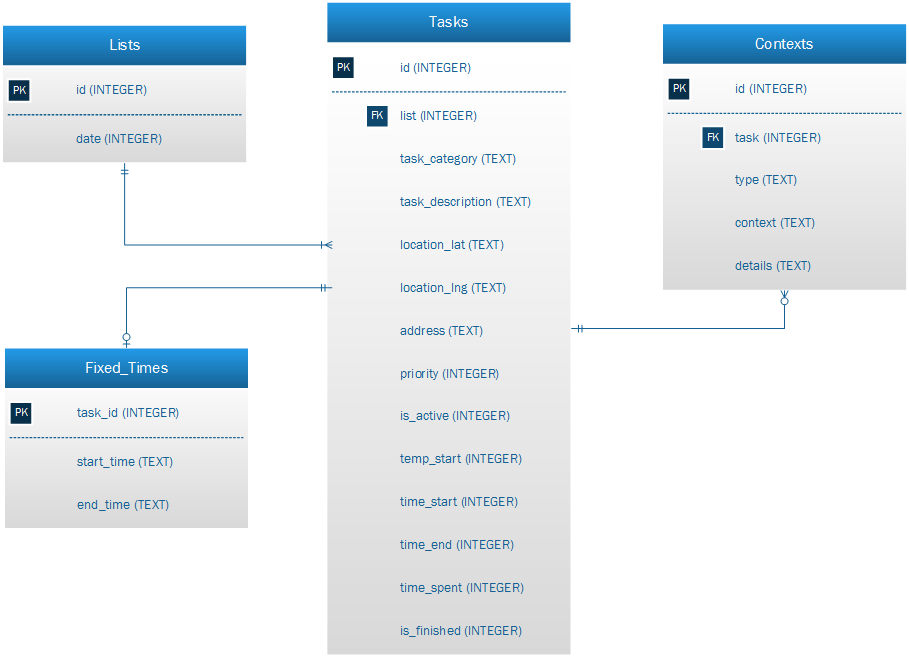
\includegraphics[width=0.8\textwidth]{figures/DatabaseModel.png}
  \caption[Database model]{SQLite representation of the individual installations application data.}
  \label{fig:databasemodel}
\end{figure}
\begin{figure}[tbp]
  \centering
  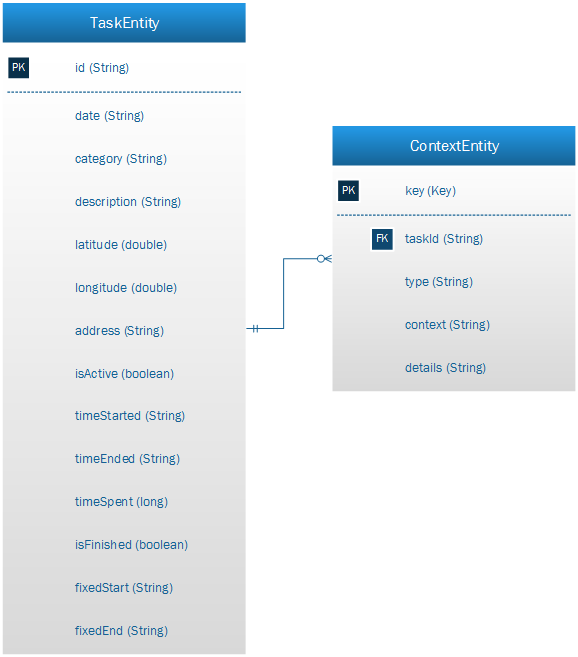
\includegraphics[width=0.5\textwidth]{figures/DatabaseModel_external.png}
  \caption[External database model]{The Google AppEngine datastore representation for all installations application data.}
  \label{fig:databasemodelexternal}
\end{figure}
The actual tasks are held in the table \emph{Task}. Each task is tied to a specific list, represented by the \emph{List} table. As a task can have an optional fixed starting and/or end time, we pulled these values out of the Task table and into the \emph{Fixed Time} table. All the collected contexts related to the tasks are held in the \emph{Context} table. The remote datastore is not normalized however, as there is no primary or foreign keys in the AppEngine datastore. This is not important, as the application only writes to the remote datastore.

The actual collection of the context data happens when the users starts a task from the application. A background service is then started and runs on the device until the task is paused by the user or completed. The service collects these contexts at certain intervals. A service to run in the background was needed in order to continuously collect contexts without disturbing the user. The user is also not actively using the mobile device when performing a task, so by implementing a service we could collect contexts even when the device is in an idle state. If a collected context, for example location, is already collected for a specific task then that context is not stored again. Multiple identical locations for a single task is not needed, so this prevents some information overhead.



\section{Recommender}
\label{sec:recommender}

When creating the recommender part of the application, several decisions needed to be made. First of all, we needed to decide what kind of recommendations to make. There where many possible ways to do this:
\begin{itemize}
	\item Location proximity recommendations.
  \item Recommendations based on time of day.
  \item Recommendations based on time spent on previous tasks.
  \item Recommend tasks with fixed starting times.
  \item Recommend tasks based on the shortest traveling distance between tasks.
  \item Recommendations based on regularity of task occurrences.
  \item Combinations of the above.
\end{itemize}

After deciding what to recommend, the underlying logic also needed to be decided. A recommender will need some form of logic for comparison, so that it can know that it should recommend one task over another. Such logic already exist in some systems. We have seen Netflix\cite{netflix} recommend movies and Amazon\cite{amazon} recommend books to name a couple. It is potentially beneficial to analyze other systems for reusable recommendation algorithms.


\subsection{Chosen recommendation algorithm}
Implementing a recommender algorithm based on neural networks would require a lot of work, probably more than what can be achieved in the scope of this thesis. By using probability calculations however, we can create much simpler mathematical formulas to calculate the probability of different tasks. This is the approach that was used in this thesis. As mentioned earlier, the input for the recommender consists of the user's planned tasks, the current context, and the entire task history with related contexts. The recommender starts by looking at the categories of the user's planned tasks and tries to calculate a probability for each of them, representing how likely the task is going to be chosen next by the user. This calculation is done based on the tasks that the user has previously done and in what contexts. Probability calculations are made individually for each of the different contexts, but also for combinations of them. The probability for a specific task is calculated by following the following formula:
$$
  P(t(ca)) = \frac{\sum_{i=1}^{n}t_i(ca)}{\sum_{i=1}^{n}t_i(c)}
$$
t(ca) represents a task that matches a given category and context and t(c) represents a task that matches the given context. We then get the probability P(TC) of a task category. In other words, the probability represents the relationship between all tasks of a given category and context, and all tasks with the given context.

As an example, the recommender could consider the current time of day. The recommender will then find other tasks that have been done during the same time of day previously. By dividing the total number of a particular task category performed at that time of day by the total number of tasks performed at the same time of day, we get the probability for a task category for that time of day. This is done for each of the task categories that the user has planned and the result is put into a map, as shown in Table~\ref{tab:probabilitymaptimeofday}.
\begin{table}[tbp]
  \centering
  \begin{tabular}{|l|r|}
	\hline
	\textbf{Task category} & \textbf{Probability} \\
	\hline
	Attend lecture & 0.11 \\
  \hline
	Other & 0.24 \\
	\hline
	Practical work & 0.46 \\
	\hline
	Read & 0.14 \\
	\hline
	Write report & 0.05 \\
	\hline
  \end{tabular}
  \caption{Example recommendation probability hashmap}
  \label{tab:probabilitymaptimeofday}
\end{table}

The same process is executed for other contexts as well. For example, based on the current location of the user, the recommender finds all tasks that have been performed in that particular location. Probabilities are then calculated the same way as for the time of day. The task probability map based on location may look like Table~\ref{tab:probabilitymaplocation}.
\begin{table}[tbp]
  \centering
  \begin{tabular}{|l|r|}
	\hline
	\textbf{Task category} & \textbf{Probability} \\
	\hline
	Attend lecture & 0.41 \\
	\hline
	Other & 0.13 \\
	\hline
	Practical work & 0.25 \\
	\hline
	Read & 0.16 \\
	\hline
	Write report & 0.05 \\
	\hline
  \end{tabular}
  \caption{Location recommendation probability hashmap}
  \label{tab:probabilitymaplocation}
\end{table}

Similar maps are calculated for each context and all combinations of them. This means:
\begin{itemize}
	\item Time of day
	\item Day of week
	\item Location
	\item Time of day \emph{and} location
	\item Time of day \emph{and} day of week
	\item Day of week \emph{and} location
	\item Time of day \emph{and} day of week \emph{and} location
\end{itemize}
The highest probability from each of these individual probability maps are then put into a resulting map, where the highest probability in this map will be the actual task recommendation made by the recommender. Looking at Table~\ref{tab:probabilitymaptimeofday} and Table~\ref{tab:probabilitymaplocation}, the resulting map will look like Table~\ref{tab:probabilitymapresult}.
\begin{table}[tbp]
  \centering
  \begin{tabular}{|l|r|}
	\hline
	\textbf{Task category} & \textbf{Probability} \\
	\hline
	Attend lecture & 0.41 \\
	\hline
	Practical work & 0.46 \\
	\hline
  \end{tabular}
  \caption{Resulting probability hashmap upon which the actual recommendation is made}
  \label{tab:probabilitymapresult}
\end{table}
The actual recommendation made by the recommender in this example would be the task with the category ``practical work''.

\section{Application distribution and user experiments}
To test our design decision we needed users to test the application for a certain period of time. Because the application is based on task and context history, it would take some time and usage in order for history to build up. A large history of tasks and contexts is needed so that for the recommender can make reasonable recommendations. The recommendations from the recommender should increase in accuracy over time. By accuracy we mean tasks that matches the tasks that the users intend to do next. We could say that the application is ``learning'' the users behavior over time. For this experiment, we considered 2-3 weeks to be enough time to get some useful data from the application usage. Ideally the experiment would run over an even longer period, but having a timeframe for this thesis a maximum timeframe for the experimenting needed to be set.

The application was uploaded to Google Play for distributing. This made the application easily available for anyone who wished to test it. Requesting participants for the application testing was done by mailing students at Gjøvik University College. The application was found by following the link provided by mail, or searching for ``Todoity'' in Google Play.